\documentclass[1p]{elsarticle_modified}
%\bibliographystyle{elsarticle-num}

%\usepackage[colorlinks]{hyperref}
%\usepackage{abbrmath_seonhwa} %\Abb, \Ascr, \Acal ,\Abf, \Afrak
\usepackage{amsfonts}
\usepackage{amssymb}
\usepackage{amsmath}
\usepackage{amsthm}
\usepackage{scalefnt}
\usepackage{amsbsy}
\usepackage{kotex}
\usepackage{caption}
\usepackage{subfig}
\usepackage{color}
\usepackage{graphicx}
\usepackage{xcolor} %% white, black, red, green, blue, cyan, magenta, yellow
\usepackage{float}
\usepackage{setspace}
\usepackage{hyperref}

\usepackage{tikz}
\usetikzlibrary{arrows}

\usepackage{multirow}
\usepackage{array} % fixed length table
\usepackage{hhline}

%%%%%%%%%%%%%%%%%%%%%
\makeatletter
\renewcommand*\env@matrix[1][\arraystretch]{%
	\edef\arraystretch{#1}%
	\hskip -\arraycolsep
	\let\@ifnextchar\new@ifnextchar
	\array{*\c@MaxMatrixCols c}}
\makeatother %https://tex.stackexchange.com/questions/14071/how-can-i-increase-the-line-spacing-in-a-matrix
%%%%%%%%%%%%%%%

\usepackage[normalem]{ulem}

\newcommand{\msout}[1]{\ifmmode\text{\sout{\ensuremath{#1}}}\else\sout{#1}\fi}
%SOURCE: \msout is \stkout macro in https://tex.stackexchange.com/questions/20609/strikeout-in-math-mode

\newcommand{\cancel}[1]{
	\ifmmode
	{\color{red}\msout{#1}}
	\else
	{\color{red}\sout{#1}}
	\fi
}

\newcommand{\add}[1]{
	{\color{blue}\uwave{#1}}
}

\newcommand{\replace}[2]{
	\ifmmode
	{\color{red}\msout{#1}}{\color{blue}\uwave{#2}}
	\else
	{\color{red}\sout{#1}}{\color{blue}\uwave{#2}}
	\fi
}

\newcommand{\Sol}{\mathcal{S}} %segment
\newcommand{\D}{D} %diagram
\newcommand{\A}{\mathcal{A}} %arc


%%%%%%%%%%%%%%%%%%%%%%%%%%%%%5 test

\def\sl{\operatorname{\textup{SL}}(2,\Cbb)}
\def\psl{\operatorname{\textup{PSL}}(2,\Cbb)}
\def\quan{\mkern 1mu \triangleright \mkern 1mu}

\theoremstyle{definition}
\newtheorem{thm}{Theorem}[section]
\newtheorem{prop}[thm]{Proposition}
\newtheorem{lem}[thm]{Lemma}
\newtheorem{ques}[thm]{Question}
\newtheorem{cor}[thm]{Corollary}
\newtheorem{defn}[thm]{Definition}
\newtheorem{exam}[thm]{Example}
\newtheorem{rmk}[thm]{Remark}
\newtheorem{alg}[thm]{Algorithm}

\newcommand{\I}{\sqrt{-1}}
\begin{document}

%\begin{frontmatter}
%
%\title{Boundary parabolic representations of knots up to 8 crossings}
%
%%% Group authors per affiliation:
%\author{Yunhi Cho} 
%\address{Department of Mathematics, University of Seoul, Seoul, Korea}
%\ead{yhcho@uos.ac.kr}
%
%
%\author{Seonhwa Kim} %\fnref{s_kim}}
%\address{Center for Geometry and Physics, Institute for Basic Science, Pohang, 37673, Korea}
%\ead{ryeona17@ibs.re.kr}
%
%\author{Hyuk Kim}
%\address{Department of Mathematical Sciences, Seoul National University, Seoul 08826, Korea}
%\ead{hyukkim@snu.ac.kr}
%
%\author{Seokbeom Yoon}
%\address{Department of Mathematical Sciences, Seoul National University, Seoul, 08826,  Korea}
%\ead{sbyoon15@snu.ac.kr}
%
%\begin{abstract}
%We find all boundary parabolic representation of knots up to 8 crossings.
%
%\end{abstract}
%\begin{keyword}
%    \MSC[2010] 57M25 
%\end{keyword}
%
%\end{frontmatter}

%\linenumbers
%\tableofcontents
%
\newcommand\colored[1]{\textcolor{white}{\rule[-0.35ex]{0.8em}{1.4ex}}\kern-0.8em\color{red} #1}%
%\newcommand\colored[1]{\textcolor{white}{ #1}\kern-2.17ex	\textcolor{white}{ #1}\kern-1.81ex	\textcolor{white}{ #1}\kern-2.15ex\color{red}#1	}

{\Large $\underline{11a_{327}~(K11a_{327})}$}

\setlength{\tabcolsep}{10pt}
\renewcommand{\arraystretch}{1.6}
\vspace{1cm}\begin{tabular}{m{100pt}>{\centering\arraybackslash}m{274pt}}
\multirow{5}{120pt}{
	\centering
	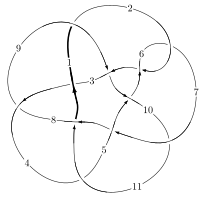
\includegraphics[width=112pt]{../../../GIT/diagram.site/Diagrams/png/576_11a_327.png}\\
\ \ \ A knot diagram\footnotemark}&
\allowdisplaybreaks
\textbf{Linearized knot diagam} \\
\cline{2-2}
 &
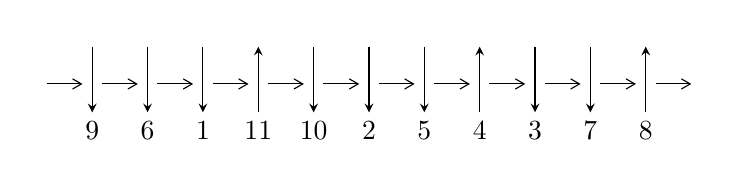
\begin{tikzpicture}[x=20pt, y=17pt]
	% nodes
	\node (C0) at (0, 0) {};
	\node (C1) at (1, 0) {};
	\node (C1U) at (1, +1) {};
	\node (C1D) at (1, -1) {9};

	\node (C2) at (2, 0) {};
	\node (C2U) at (2, +1) {};
	\node (C2D) at (2, -1) {6};

	\node (C3) at (3, 0) {};
	\node (C3U) at (3, +1) {};
	\node (C3D) at (3, -1) {1};

	\node (C4) at (4, 0) {};
	\node (C4U) at (4, +1) {};
	\node (C4D) at (4, -1) {11};

	\node (C5) at (5, 0) {};
	\node (C5U) at (5, +1) {};
	\node (C5D) at (5, -1) {10};

	\node (C6) at (6, 0) {};
	\node (C6U) at (6, +1) {};
	\node (C6D) at (6, -1) {2};

	\node (C7) at (7, 0) {};
	\node (C7U) at (7, +1) {};
	\node (C7D) at (7, -1) {5};

	\node (C8) at (8, 0) {};
	\node (C8U) at (8, +1) {};
	\node (C8D) at (8, -1) {4};

	\node (C9) at (9, 0) {};
	\node (C9U) at (9, +1) {};
	\node (C9D) at (9, -1) {3};

	\node (C10) at (10, 0) {};
	\node (C10U) at (10, +1) {};
	\node (C10D) at (10, -1) {7};

	\node (C11) at (11, 0) {};
	\node (C11U) at (11, +1) {};
	\node (C11D) at (11, -1) {8};
	\node (C12) at (12, 0) {};

	% arrows
	\draw[->,>={angle 60}]
	(C0) edge (C1) (C1) edge (C2) (C2) edge (C3) (C3) edge (C4) (C4) edge (C5) (C5) edge (C6) (C6) edge (C7) (C7) edge (C8) (C8) edge (C9) (C9) edge (C10) (C10) edge (C11) (C11) edge (C12) ;	\draw[->,>=stealth]
	(C1U) edge (C1D) (C2U) edge (C2D) (C3U) edge (C3D) (C4D) edge (C4U) (C5U) edge (C5D) (C6U) edge (C6D) (C7U) edge (C7D) (C8D) edge (C8U) (C9U) edge (C9D) (C10U) edge (C10D) (C11D) edge (C11U) ;
	\end{tikzpicture} \\
\hhline{~~} \\& 
\textbf{Solving Sequence} \\ \cline{2-2} 
 &
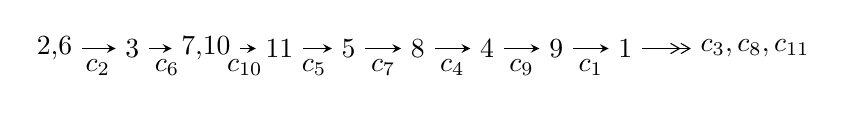
\begin{tikzpicture}[x=25pt, y=7pt]
	% node
	\node (A0) at (-1/8, 0) {2,6};
	\node (A1) at (1, 0) {3};
	\node (A2) at (33/16, 0) {7,10};
	\node (A3) at (25/8, 0) {11};
	\node (A4) at (33/8, 0) {5};
	\node (A5) at (41/8, 0) {8};
	\node (A6) at (49/8, 0) {4};
	\node (A7) at (57/8, 0) {9};
	\node (A8) at (65/8, 0) {1};
	\node (C1) at (1/2, -1) {$c_{2}$};
	\node (C2) at (3/2, -1) {$c_{6}$};
	\node (C3) at (21/8, -1) {$c_{10}$};
	\node (C4) at (29/8, -1) {$c_{5}$};
	\node (C5) at (37/8, -1) {$c_{7}$};
	\node (C6) at (45/8, -1) {$c_{4}$};
	\node (C7) at (53/8, -1) {$c_{9}$};
	\node (C8) at (61/8, -1) {$c_{1}$};
	\node (A9) at (10, 0) {$c_{3},c_{8},c_{11}$};

	% edge
	\draw[->,>=stealth]	
	(A0) edge (A1) (A1) edge (A2) (A2) edge (A3) (A3) edge (A4) (A4) edge (A5) (A5) edge (A6) (A6) edge (A7) (A7) edge (A8) ;
	\draw[->>,>={angle 60}]	
	(A8) edge (A9);
\end{tikzpicture} \\ 

\end{tabular} \\

\footnotetext{
The image of knot diagram is generated by the software ``\textbf{Draw programme}" developed by Andrew Bartholomew(\url{http://www.layer8.co.uk/maths/draw/index.htm\#Running-draw}), where we modified some parts for our purpose(\url{https://github.com/CATsTAILs/LinksPainter}).
}\phantom \\ \newline 
\centering \textbf{Ideals for irreducible components\footnotemark of $X_{\text{par}}$} 
 
\begin{align*}
I^u_{1}&=\langle 
4427228 u^{24}-51386293 u^{23}+\cdots+7423256 b+218726992,\\
\phantom{I^u_{1}}&\phantom{= \langle  }-5223503 u^{24}+65905467 u^{23}+\cdots+14846512 a-424794688,\;u^{25}-11 u^{24}+\cdots+304 u-32\rangle \\
I^u_{2}&=\langle 
-487 u^{15}-1824 u^{14}+\cdots+1084 b-1471,\;1589 u^{15}+3060 u^{14}+\cdots+1084 a-2223,\\
\phantom{I^u_{2}}&\phantom{= \langle  }u^{16}+2 u^{15}+6 u^{14}+8 u^{13}+10 u^{12}+13 u^{11}+7 u^{10}+15 u^9+5 u^8+8 u^7+9 u^6-4 u^5+12 u^4-6 u^3+7 u^2- u+1\rangle \\
I^u_{3}&=\langle 
-232 u^{41}-1201 u^{40}+\cdots+16 b-31,\;31 u^{41} a+170 u^{41}+\cdots-515 a+1252,\;u^{42}+6 u^{41}+\cdots+5 u-1\rangle \\
\\
\end{align*}
\raggedright * 3 irreducible components of $\dim_{\mathbb{C}}=0$, with total 125 representations.\\
\footnotetext{All coefficients of polynomials are rational numbers. But the coefficients are sometimes approximated in decimal forms when there is not enough margin.}
\newpage
\renewcommand{\arraystretch}{1}
\centering \section*{I. $I^u_{1}= \langle 4.43\times10^{6} u^{24}-5.14\times10^{7} u^{23}+\cdots+7.42\times10^{6} b+2.19\times10^{8},\;-5.22\times10^{6} u^{24}+6.59\times10^{7} u^{23}+\cdots+1.48\times10^{7} a-4.25\times10^{8},\;u^{25}-11 u^{24}+\cdots+304 u-32 \rangle$}
\flushleft \textbf{(i) Arc colorings}\\
\begin{tabular}{m{7pt} m{180pt} m{7pt} m{180pt} }
\flushright $a_{2}=$&$\begin{pmatrix}1\\0\end{pmatrix}$ \\
\flushright $a_{6}=$&$\begin{pmatrix}0\\u\end{pmatrix}$ \\
\flushright $a_{3}=$&$\begin{pmatrix}1\\u^2\end{pmatrix}$ \\
\flushright $a_{7}=$&$\begin{pmatrix}- u\\u\end{pmatrix}$ \\
\flushright $a_{10}=$&$\begin{pmatrix}0.351834 u^{24}-4.43912 u^{23}+\cdots-244.548 u+28.6124\\-0.596400 u^{24}+6.92234 u^{23}+\cdots+262.565 u-29.4651\end{pmatrix}$ \\
\flushright $a_{11}=$&$\begin{pmatrix}0.311972 u^{24}-4.00378 u^{23}+\cdots-299.653 u+35.2367\\-0.556538 u^{24}+6.48700 u^{23}+\cdots+317.669 u-36.0894\end{pmatrix}$ \\
\flushright $a_{5}=$&$\begin{pmatrix}-0.250673 u^{24}+3.42364 u^{23}+\cdots+197.791 u-19.2950\\0.161063 u^{24}-2.76565 u^{23}+\cdots-266.465 u+29.3409\end{pmatrix}$ \\
\flushright $a_{8}=$&$\begin{pmatrix}-0.277406 u^{24}+3.01578 u^{23}+\cdots+199.144 u-23.7794\\-0.0363785 u^{24}+0.0499409 u^{23}+\cdots-154.341 u+18.2222\end{pmatrix}$ \\
\flushright $a_{4}=$&$\begin{pmatrix}0.235672 u^{24}-2.80148 u^{23}+\cdots-87.9695 u+9.74840\\-0.130974 u^{24}+1.51883 u^{23}+\cdots-18.7296 u+3.35035\end{pmatrix}$ \\
\flushright $a_{9}=$&$\begin{pmatrix}0.920784 u^{24}-9.53223 u^{23}+\cdots-166.203 u+17.3537\\0.207009 u^{24}-2.31696 u^{23}+\cdots-73.4954 u+7.82611\end{pmatrix}$ \\
\flushright $a_{1}=$&$\begin{pmatrix}0.238111 u^{24}-2.57557 u^{23}+\cdots-106.961 u+13.9134\\0.163550 u^{24}-1.64723 u^{23}+\cdots-42.9394 u+4.26453\end{pmatrix}$\\ \flushright $a_{1}=$&$\begin{pmatrix}0.238111 u^{24}-2.57557 u^{23}+\cdots-106.961 u+13.9134\\0.163550 u^{24}-1.64723 u^{23}+\cdots-42.9394 u+4.26453\end{pmatrix}$\\&\end{tabular}
\flushleft \textbf{(ii) Obstruction class $= -1$}\\~\\
\flushleft \textbf{(iii) Cusp Shapes $= \frac{4915601}{1855814} u^{24}-\frac{53210001}{1855814} u^{23}+\cdots-\frac{95751464}{927907} u-\frac{19294134}{927907}$}\\~\\
\newpage\renewcommand{\arraystretch}{1}
\flushleft \textbf{(iv) u-Polynomials at the component}\newline \\
\begin{tabular}{m{50pt}|m{274pt}}
Crossings & \hspace{64pt}u-Polynomials at each crossing \\
\hline $$\begin{aligned}c_{1},c_{10}\end{aligned}$$&$\begin{aligned}
&u^{25}-2 u^{24}+\cdots-5 u+1
\end{aligned}$\\
\hline $$\begin{aligned}c_{2},c_{6}\end{aligned}$$&$\begin{aligned}
&u^{25}+11 u^{24}+\cdots+304 u+32
\end{aligned}$\\
\hline $$\begin{aligned}c_{3},c_{7}\end{aligned}$$&$\begin{aligned}
&u^{25}-2 u^{24}+\cdots-7 u+1
\end{aligned}$\\
\hline $$\begin{aligned}c_{4},c_{8}\end{aligned}$$&$\begin{aligned}
&u^{25}-6 u^{24}+\cdots+2 u+1
\end{aligned}$\\
\hline $$\begin{aligned}c_{5},c_{9}\end{aligned}$$&$\begin{aligned}
&u^{25}-6 u^{24}+\cdots+13 u^2+1
\end{aligned}$\\
\hline $$\begin{aligned}c_{11}\end{aligned}$$&$\begin{aligned}
&u^{25}-18 u^{24}+\cdots-1536 u+256
\end{aligned}$\\
\hline
\end{tabular}\\~\\
\newpage\renewcommand{\arraystretch}{1}
\flushleft \textbf{(v) Riley Polynomials at the component}\newline \\
\begin{tabular}{m{50pt}|m{274pt}}
Crossings & \hspace{64pt}Riley Polynomials at each crossing \\
\hline $$\begin{aligned}c_{1},c_{10}\end{aligned}$$&$\begin{aligned}
&y^{25}+6 y^{24}+\cdots-9 y-1
\end{aligned}$\\
\hline $$\begin{aligned}c_{2},c_{6}\end{aligned}$$&$\begin{aligned}
&y^{25}+11 y^{24}+\cdots-3328 y-1024
\end{aligned}$\\
\hline $$\begin{aligned}c_{3},c_{7}\end{aligned}$$&$\begin{aligned}
&y^{25}+22 y^{23}+\cdots+17 y-1
\end{aligned}$\\
\hline $$\begin{aligned}c_{4},c_{8}\end{aligned}$$&$\begin{aligned}
&y^{25}-2 y^{24}+\cdots-16 y-1
\end{aligned}$\\
\hline $$\begin{aligned}c_{5},c_{9}\end{aligned}$$&$\begin{aligned}
&y^{25}+4 y^{24}+\cdots-26 y-1
\end{aligned}$\\
\hline $$\begin{aligned}c_{11}\end{aligned}$$&$\begin{aligned}
&y^{25}+10 y^{24}+\cdots+720896 y-65536
\end{aligned}$\\
\hline
\end{tabular}\\~\\
\newpage\flushleft \textbf{(vi) Complex Volumes and Cusp Shapes}
$$\begin{array}{c|c|c}  
\text{Solutions to }I^u_{1}& \I (\text{vol} + \sqrt{-1}CS) & \text{Cusp shape}\\
 \hline 
\begin{aligned}
u &= \phantom{-}0.415596 + 0.889012 I \\
a &= -1.53371 + 1.85229 I \\
b &= \phantom{-}1.86263 - 1.68366 I\end{aligned}
 & \phantom{-}1.61415 - 1.93498 I & -3.0424 + 31.4661 I \\ \hline\begin{aligned}
u &= \phantom{-}0.415596 - 0.889012 I \\
a &= -1.53371 - 1.85229 I \\
b &= \phantom{-}1.86263 + 1.68366 I\end{aligned}
 & \phantom{-}1.61415 + 1.93498 I & -3.0424 - 31.4661 I \\ \hline\begin{aligned}
u &= \phantom{-}1.003880 + 0.591915 I \\
a &= -0.060664 + 0.510320 I \\
b &= -0.283392 - 0.212996 I\end{aligned}
 & -2.76859 - 1.48183 I & -6.65987 - 5.81420 I \\ \hline\begin{aligned}
u &= \phantom{-}1.003880 - 0.591915 I \\
a &= -0.060664 - 0.510320 I \\
b &= -0.283392 + 0.212996 I\end{aligned}
 & -2.76859 + 1.48183 I & -6.65987 + 5.81420 I \\ \hline\begin{aligned}
u &= -1.142140 + 0.259514 I \\
a &= -0.132195 + 0.169180 I \\
b &= -0.170331 + 0.515196 I\end{aligned}
 & -1.89203 + 4.73023 I & -8.60021 - 1.58329 I \\ \hline\begin{aligned}
u &= -1.142140 - 0.259514 I \\
a &= -0.132195 - 0.169180 I \\
b &= -0.170331 - 0.515196 I\end{aligned}
 & -1.89203 - 4.73023 I & -8.60021 + 1.58329 I \\ \hline\begin{aligned}
u &= \phantom{-}1.142400 + 0.260296 I \\
a &= \phantom{-}0.360462 - 1.041080 I \\
b &= \phantom{-}0.382380 + 0.021730 I\end{aligned}
 & \phantom{-}0.01107 + 12.92330 I & -4.84732 - 8.19604 I \\ \hline\begin{aligned}
u &= \phantom{-}1.142400 - 0.260296 I \\
a &= \phantom{-}0.360462 + 1.041080 I \\
b &= \phantom{-}0.382380 - 0.021730 I\end{aligned}
 & \phantom{-}0.01107 - 12.92330 I & -4.84732 + 8.19604 I \\ \hline\begin{aligned}
u &= \phantom{-}0.071145 + 1.245000 I \\
a &= -0.926069 + 0.287044 I \\
b &= \phantom{-}1.80314 + 0.52501 I\end{aligned}
 & \phantom{-}6.44614 - 2.45412 I & \phantom{-}2.40382 + 6.69375 I \\ \hline\begin{aligned}
u &= \phantom{-}0.071145 - 1.245000 I \\
a &= -0.926069 - 0.287044 I \\
b &= \phantom{-}1.80314 - 0.52501 I\end{aligned}
 & \phantom{-}6.44614 + 2.45412 I & \phantom{-}2.40382 - 6.69375 I\\
 \hline 
 \end{array}$$\newpage$$\begin{array}{c|c|c}  
\text{Solutions to }I^u_{1}& \I (\text{vol} + \sqrt{-1}CS) & \text{Cusp shape}\\
 \hline 
\begin{aligned}
u &= \phantom{-}1.263360 + 0.222570 I \\
a &= -0.217471 + 0.724765 I \\
b &= -0.307861 + 0.131345 I\end{aligned}
 & -2.66023 + 4.12938 I & -8.27327 - 5.73297 I \\ \hline\begin{aligned}
u &= \phantom{-}1.263360 - 0.222570 I \\
a &= -0.217471 - 0.724765 I \\
b &= -0.307861 - 0.131345 I\end{aligned}
 & -2.66023 - 4.12938 I & -8.27327 + 5.73297 I \\ \hline\begin{aligned}
u &= \phantom{-}0.634694 + 1.156470 I \\
a &= \phantom{-}0.870338 - 0.021834 I \\
b &= -1.358990 + 0.305406 I\end{aligned}
 & -0.75795 - 4.50706 I & -7.57070 + 5.07072 I \\ \hline\begin{aligned}
u &= \phantom{-}0.634694 - 1.156470 I \\
a &= \phantom{-}0.870338 + 0.021834 I \\
b &= -1.358990 - 0.305406 I\end{aligned}
 & -0.75795 + 4.50706 I & -7.57070 - 5.07072 I \\ \hline\begin{aligned}
u &= \phantom{-}0.63878 + 1.29685 I \\
a &= -1.205210 + 0.103104 I \\
b &= \phantom{-}2.26792 - 0.63100 I\end{aligned}
 & \phantom{-}3.3047 - 19.2356 I & -2.92755 + 10.21183 I \\ \hline\begin{aligned}
u &= \phantom{-}0.63878 - 1.29685 I \\
a &= -1.205210 - 0.103104 I \\
b &= \phantom{-}2.26792 + 0.63100 I\end{aligned}
 & \phantom{-}3.3047 + 19.2356 I & -2.92755 - 10.21183 I \\ \hline\begin{aligned}
u &= \phantom{-}0.20692 + 1.46356 I \\
a &= \phantom{-}0.639225 + 0.048922 I \\
b &= -1.43216 - 0.66120 I\end{aligned}
 & \phantom{-}6.31210 + 7.97978 I & \phantom{-}0.59190 - 6.19914 I \\ \hline\begin{aligned}
u &= \phantom{-}0.20692 - 1.46356 I \\
a &= \phantom{-}0.639225 - 0.048922 I \\
b &= -1.43216 + 0.66120 I\end{aligned}
 & \phantom{-}6.31210 - 7.97978 I & \phantom{-}0.59190 + 6.19914 I \\ \hline\begin{aligned}
u &= \phantom{-}0.139855 + 0.499323 I \\
a &= \phantom{-}0.65973 + 1.57256 I \\
b &= \phantom{-}0.321732 - 0.818524 I\end{aligned}
 & \phantom{-}1.59913 - 1.70507 I & \phantom{-}2.11756 + 1.16667 I \\ \hline\begin{aligned}
u &= \phantom{-}0.139855 - 0.499323 I \\
a &= \phantom{-}0.65973 - 1.57256 I \\
b &= \phantom{-}0.321732 + 0.818524 I\end{aligned}
 & \phantom{-}1.59913 + 1.70507 I & \phantom{-}2.11756 - 1.16667 I\\
 \hline 
 \end{array}$$\newpage$$\begin{array}{c|c|c}  
\text{Solutions to }I^u_{1}& \I (\text{vol} + \sqrt{-1}CS) & \text{Cusp shape}\\
 \hline 
\begin{aligned}
u &= \phantom{-}0.64308 + 1.34654 I \\
a &= \phantom{-}1.001290 - 0.082426 I \\
b &= -2.01357 + 0.55420 I\end{aligned}
 & \phantom{-}0.99069 - 10.76890 I & -7.04060 + 8.50753 I \\ \hline\begin{aligned}
u &= \phantom{-}0.64308 - 1.34654 I \\
a &= \phantom{-}1.001290 + 0.082426 I \\
b &= -2.01357 - 0.55420 I\end{aligned}
 & \phantom{-}0.99069 + 10.76890 I & -7.04060 - 8.50753 I \\ \hline\begin{aligned}
u &= \phantom{-}0.25168 + 1.49957 I \\
a &= -0.606065 + 0.151895 I \\
b &= \phantom{-}1.59013 + 0.08120 I\end{aligned}
 & \phantom{-}3.88935 - 1.44009 I & -9.35211 + 8.90381 I \\ \hline\begin{aligned}
u &= \phantom{-}0.25168 - 1.49957 I \\
a &= -0.606065 - 0.151895 I \\
b &= \phantom{-}1.59013 - 0.08120 I\end{aligned}
 & \phantom{-}3.88935 + 1.44009 I & -9.35211 - 8.90381 I \\ \hline\begin{aligned}
u &= \phantom{-}0.461512\phantom{ +0.000000I} \\
a &= \phantom{-}1.30067\phantom{ +0.000000I} \\
b &= -0.323241\phantom{ +0.000000I}\end{aligned}
 & -0.923370\phantom{ +0.000000I} & -10.5990\phantom{ +0.000000I}\\
 \hline 
 \end{array}$$\newpage\newpage\renewcommand{\arraystretch}{1}
\centering \section*{II. $I^u_{2}= \langle -487 u^{15}-1824 u^{14}+\cdots+1084 b-1471,\;1589 u^{15}+3060 u^{14}+\cdots+1084 a-2223,\;u^{16}+2 u^{15}+\cdots- u+1 \rangle$}
\flushleft \textbf{(i) Arc colorings}\\
\begin{tabular}{m{7pt} m{180pt} m{7pt} m{180pt} }
\flushright $a_{2}=$&$\begin{pmatrix}1\\0\end{pmatrix}$ \\
\flushright $a_{6}=$&$\begin{pmatrix}0\\u\end{pmatrix}$ \\
\flushright $a_{3}=$&$\begin{pmatrix}1\\u^2\end{pmatrix}$ \\
\flushright $a_{7}=$&$\begin{pmatrix}- u\\u\end{pmatrix}$ \\
\flushright $a_{10}=$&$\begin{pmatrix}-1.46587 u^{15}-2.82288 u^{14}+\cdots-8.94373 u+2.05074\\0.449262 u^{15}+1.68266 u^{14}+\cdots+2.15959 u+1.35701\end{pmatrix}$ \\
\flushright $a_{11}=$&$\begin{pmatrix}-2.16513 u^{15}-4.00554 u^{14}+\cdots-10.8533 u+2.94373\\1.14852 u^{15}+2.86531 u^{14}+\cdots+4.06919 u+0.464022\end{pmatrix}$ \\
\flushright $a_{5}=$&$\begin{pmatrix}-1.54520 u^{15}-1.93727 u^{14}+\cdots-11.4124 u+3.55443\\1.44557 u^{15}+2.59594 u^{14}+\cdots+5.70756 u+0.392066\end{pmatrix}$ \\
\flushright $a_{8}=$&$\begin{pmatrix}0.904982 u^{15}+0.642066 u^{14}+\cdots+6.23524 u-5.72232\\-1.47325 u^{15}-2.99631 u^{14}+\cdots-6.84779 u+1.12085\end{pmatrix}$ \\
\flushright $a_{4}=$&$\begin{pmatrix}1.52768 u^{15}+4.90037 u^{14}+\cdots+2.14022 u+5.48708\\0.885609 u^{15}+0.811808 u^{14}+\cdots+5.48708 u-2.41328\end{pmatrix}$ \\
\flushright $a_{9}=$&$\begin{pmatrix}-1.35701 u^{15}-2.26476 u^{14}+\cdots-8.35886 u+3.51661\\0.892989 u^{15}+2.48524 u^{14}+\cdots+2.39114 u+1.01661\end{pmatrix}$ \\
\flushright $a_{1}=$&$\begin{pmatrix}-0.758303 u^{15}-2.07011 u^{14}+\cdots+2.85793 u-3.04613\\-0.258303 u^{15}-0.0701107 u^{14}+\cdots-3.64207 u+0.453875\end{pmatrix}$\\ \flushright $a_{1}=$&$\begin{pmatrix}-0.758303 u^{15}-2.07011 u^{14}+\cdots+2.85793 u-3.04613\\-0.258303 u^{15}-0.0701107 u^{14}+\cdots-3.64207 u+0.453875\end{pmatrix}$\\&\end{tabular}
\flushleft \textbf{(ii) Obstruction class $= 1$}\\~\\
\flushleft \textbf{(iii) Cusp Shapes $= \frac{883}{271} u^{15}+\frac{7393}{1084} u^{14}+\cdots+\frac{7220}{271} u-\frac{8893}{1084}$}\\~\\
\newpage\renewcommand{\arraystretch}{1}
\flushleft \textbf{(iv) u-Polynomials at the component}\newline \\
\begin{tabular}{m{50pt}|m{274pt}}
Crossings & \hspace{64pt}u-Polynomials at each crossing \\
\hline $$\begin{aligned}c_{1},c_{10}\end{aligned}$$&$\begin{aligned}
&u^{16}+2 u^{15}+\cdots+4 u+12
\end{aligned}$\\
\hline $$\begin{aligned}c_{2}\end{aligned}$$&$\begin{aligned}
&u^{16}+2 u^{15}+\cdots- u+1
\end{aligned}$\\
\hline $$\begin{aligned}c_{3},c_{7}\end{aligned}$$&$\begin{aligned}
&u^{16}+2 u^{15}+\cdots+8 u+4
\end{aligned}$\\
\hline $$\begin{aligned}c_{4},c_{8}\end{aligned}$$&$\begin{aligned}
&4(4 u^{16}+14 u^{14}+\cdots-3 u+1)
\end{aligned}$\\
\hline $$\begin{aligned}c_{5},c_{9}\end{aligned}$$&$\begin{aligned}
&4(4 u^{16}+10 u^{14}+\cdots-5 u+1)
\end{aligned}$\\
\hline $$\begin{aligned}c_{6}\end{aligned}$$&$\begin{aligned}
&u^{16}-2 u^{15}+\cdots+u+1
\end{aligned}$\\
\hline $$\begin{aligned}c_{11}\end{aligned}$$&$\begin{aligned}
&u^{16}+5 u^{15}+\cdots-2 u+1
\end{aligned}$\\
\hline
\end{tabular}\\~\\
\newpage\renewcommand{\arraystretch}{1}
\flushleft \textbf{(v) Riley Polynomials at the component}\newline \\
\begin{tabular}{m{50pt}|m{274pt}}
Crossings & \hspace{64pt}Riley Polynomials at each crossing \\
\hline $$\begin{aligned}c_{1},c_{10}\end{aligned}$$&$\begin{aligned}
&y^{16}-2 y^{15}+\cdots-352 y+144
\end{aligned}$\\
\hline $$\begin{aligned}c_{2},c_{6}\end{aligned}$$&$\begin{aligned}
&y^{16}+8 y^{15}+\cdots+13 y+1
\end{aligned}$\\
\hline $$\begin{aligned}c_{3},c_{7}\end{aligned}$$&$\begin{aligned}
&y^{16}+4 y^{15}+\cdots+48 y+16
\end{aligned}$\\
\hline $$\begin{aligned}c_{4},c_{8}\end{aligned}$$&$\begin{aligned}
&16(16 y^{16}+112 y^{15}+\cdots+15 y+1)
\end{aligned}$\\
\hline $$\begin{aligned}c_{5},c_{9}\end{aligned}$$&$\begin{aligned}
&16(16 y^{16}+80 y^{15}+\cdots-7 y+1)
\end{aligned}$\\
\hline $$\begin{aligned}c_{11}\end{aligned}$$&$\begin{aligned}
&y^{16}+7 y^{15}+\cdots-22 y+1
\end{aligned}$\\
\hline
\end{tabular}\\~\\
\newpage\flushleft \textbf{(vi) Complex Volumes and Cusp Shapes}
$$\begin{array}{c|c|c}  
\text{Solutions to }I^u_{2}& \I (\text{vol} + \sqrt{-1}CS) & \text{Cusp shape}\\
 \hline 
\begin{aligned}
u &= \phantom{-}0.127924 + 0.951196 I \\
a &= \phantom{-}1.199100 + 0.627565 I \\
b &= -1.66156 + 0.95514 I\end{aligned}
 & \phantom{-}1.55850 - 0.57188 I & -4.03325 + 0.08278 I \\ \hline\begin{aligned}
u &= \phantom{-}0.127924 - 0.951196 I \\
a &= \phantom{-}1.199100 - 0.627565 I \\
b &= -1.66156 - 0.95514 I\end{aligned}
 & \phantom{-}1.55850 + 0.57188 I & -4.03325 - 0.08278 I \\ \hline\begin{aligned}
u &= \phantom{-}0.576501 + 0.749960 I \\
a &= \phantom{-}0.038226 + 0.569336 I \\
b &= -0.906045 + 0.258948 I\end{aligned}
 & -2.90623 - 2.39320 I & -11.15335 + 3.39673 I \\ \hline\begin{aligned}
u &= \phantom{-}0.576501 - 0.749960 I \\
a &= \phantom{-}0.038226 - 0.569336 I \\
b &= -0.906045 - 0.258948 I\end{aligned}
 & -2.90623 + 2.39320 I & -11.15335 - 3.39673 I \\ \hline\begin{aligned}
u &= -0.236683 + 1.046650 I \\
a &= -1.215370 - 0.028025 I \\
b &= \phantom{-}1.56644 - 0.63415 I\end{aligned}
 & \phantom{-}6.29877 + 0.99707 I & \phantom{-}2.79381 - 0.26391 I \\ \hline\begin{aligned}
u &= -0.236683 - 1.046650 I \\
a &= -1.215370 + 0.028025 I \\
b &= \phantom{-}1.56644 + 0.63415 I\end{aligned}
 & \phantom{-}6.29877 - 0.99707 I & \phantom{-}2.79381 + 0.26391 I \\ \hline\begin{aligned}
u &= \phantom{-}0.677411 + 0.413884 I \\
a &= -0.426400 + 0.321010 I \\
b &= -0.724338 - 0.105805 I\end{aligned}
 & -2.89915 - 2.26107 I & -9.33280 + 4.93182 I \\ \hline\begin{aligned}
u &= \phantom{-}0.677411 - 0.413884 I \\
a &= -0.426400 - 0.321010 I \\
b &= -0.724338 + 0.105805 I\end{aligned}
 & -2.89915 + 2.26107 I & -9.33280 - 4.93182 I \\ \hline\begin{aligned}
u &= -1.320930 + 0.057937 I \\
a &= -0.246952 + 0.504969 I \\
b &= -0.055825 + 0.235863 I\end{aligned}
 & -1.55964 + 5.26639 I & -1.17081 - 11.68071 I \\ \hline\begin{aligned}
u &= -1.320930 - 0.057937 I \\
a &= -0.246952 - 0.504969 I \\
b &= -0.055825 - 0.235863 I\end{aligned}
 & -1.55964 - 5.26639 I & -1.17081 + 11.68071 I\\
 \hline 
 \end{array}$$\newpage$$\begin{array}{c|c|c}  
\text{Solutions to }I^u_{2}& \I (\text{vol} + \sqrt{-1}CS) & \text{Cusp shape}\\
 \hline 
\begin{aligned}
u &= -0.475337 + 1.308180 I \\
a &= \phantom{-}0.992931 + 0.359393 I \\
b &= -1.97006 - 0.64060 I\end{aligned}
 & \phantom{-}3.22523 + 10.87130 I & -2.52543 - 9.79507 I \\ \hline\begin{aligned}
u &= -0.475337 - 1.308180 I \\
a &= \phantom{-}0.992931 - 0.359393 I \\
b &= -1.97006 + 0.64060 I\end{aligned}
 & \phantom{-}3.22523 - 10.87130 I & -2.52543 + 9.79507 I \\ \hline\begin{aligned}
u &= -0.001694 + 0.451366 I \\
a &= \phantom{-}0.26545 - 2.71413 I \\
b &= \phantom{-}1.166390 + 0.676954 I\end{aligned}
 & -1.17125 - 8.19000 I & -3.99419 + 8.09299 I \\ \hline\begin{aligned}
u &= -0.001694 - 0.451366 I \\
a &= \phantom{-}0.26545 + 2.71413 I \\
b &= \phantom{-}1.166390 - 0.676954 I\end{aligned}
 & -1.17125 + 8.19000 I & -3.99419 - 8.09299 I \\ \hline\begin{aligned}
u &= -0.34720 + 1.51741 I \\
a &= -0.606987 - 0.107433 I \\
b &= \phantom{-}1.58500 - 0.00976 I\end{aligned}
 & \phantom{-}4.03350 + 1.05064 I & -2.08398 + 8.23407 I \\ \hline\begin{aligned}
u &= -0.34720 - 1.51741 I \\
a &= -0.606987 + 0.107433 I \\
b &= \phantom{-}1.58500 + 0.00976 I\end{aligned}
 & \phantom{-}4.03350 - 1.05064 I & -2.08398 - 8.23407 I\\
 \hline 
 \end{array}$$\newpage\newpage\renewcommand{\arraystretch}{1}
\centering \section*{III. $I^u_{3}= \langle -232 u^{41}-1201 u^{40}+\cdots+16 b-31,\;31 u^{41} a+170 u^{41}+\cdots-515 a+1252,\;u^{42}+6 u^{41}+\cdots+5 u-1 \rangle$}
\flushleft \textbf{(i) Arc colorings}\\
\begin{tabular}{m{7pt} m{180pt} m{7pt} m{180pt} }
\flushright $a_{2}=$&$\begin{pmatrix}1\\0\end{pmatrix}$ \\
\flushright $a_{6}=$&$\begin{pmatrix}0\\u\end{pmatrix}$ \\
\flushright $a_{3}=$&$\begin{pmatrix}1\\u^2\end{pmatrix}$ \\
\flushright $a_{7}=$&$\begin{pmatrix}- u\\u\end{pmatrix}$ \\
\flushright $a_{10}=$&$\begin{pmatrix}a\\14.5000 u^{41}+75.0625 u^{40}+\cdots-41.8750 u+1.93750\end{pmatrix}$ \\
\flushright $a_{11}=$&$\begin{pmatrix}\frac{37}{8} u^{41}+\frac{115}{8} u^{40}+\cdots+a+\frac{191}{16}\\\frac{79}{8} u^{41}+\frac{971}{16} u^{40}+\cdots+\frac{517}{16} u-10\end{pmatrix}$ \\
\flushright $a_{5}=$&$\begin{pmatrix}-14.5000 a u^{41}-4.25000 u^{41}+\cdots-1.93750 a-10.6250\\4.62500 a u^{41}+4.68750 u^{41}+\cdots+11.9375 a-0.0625000\end{pmatrix}$ \\
\flushright $a_{8}=$&$\begin{pmatrix}10.2500 a u^{41}-0.562500 u^{41}+\cdots-3.93750 a+20.2500\\-4.43750 a u^{41}-0.687500 u^{41}+\cdots+3.68750 a-1.31250\end{pmatrix}$ \\
\flushright $a_{4}=$&$\begin{pmatrix}-9.87500 a u^{41}+2.43750 u^{41}+\cdots+9.25000 a-24.5000\\9 u^{41} a-\frac{93}{16} u^{41}+\cdots+\frac{7}{8} a-\frac{21}{16}\end{pmatrix}$ \\
\flushright $a_{9}=$&$\begin{pmatrix}\frac{29}{2} u^{41}+\frac{1201}{16} u^{40}+\cdots+a+\frac{31}{16}\\\frac{79}{8} u^{41}+\frac{971}{16} u^{40}+\cdots+\frac{517}{16} u-10\end{pmatrix}$ \\
\flushright $a_{1}=$&$\begin{pmatrix}-13.3750 a u^{41}+2.56250 u^{41}+\cdots+4.62500 a+11.3750\\8.31250 a u^{41}+4.25000 u^{41}+\cdots-5.25000 a-4.06250\end{pmatrix}$\\ \flushright $a_{1}=$&$\begin{pmatrix}-13.3750 a u^{41}+2.56250 u^{41}+\cdots+4.62500 a+11.3750\\8.31250 a u^{41}+4.25000 u^{41}+\cdots-5.25000 a-4.06250\end{pmatrix}$\\&\end{tabular}
\flushleft \textbf{(ii) Obstruction class $= -1$}\\~\\
\flushleft \textbf{(iii) Cusp Shapes $= -\frac{19}{4} u^{41}-\frac{29}{2} u^{40}+\cdots+101 u-\frac{91}{4}$}\\~\\
\newpage\renewcommand{\arraystretch}{1}
\flushleft \textbf{(iv) u-Polynomials at the component}\newline \\
\begin{tabular}{m{50pt}|m{274pt}}
Crossings & \hspace{64pt}u-Polynomials at each crossing \\
\hline $$\begin{aligned}c_{1},c_{10}\end{aligned}$$&$\begin{aligned}
&u^{84}-3 u^{83}+\cdots+3176 u+2356
\end{aligned}$\\
\hline $$\begin{aligned}c_{2},c_{6}\end{aligned}$$&$\begin{aligned}
&(u^{42}-6 u^{41}+\cdots-5 u-1)^{2}
\end{aligned}$\\
\hline $$\begin{aligned}c_{3},c_{7}\end{aligned}$$&$\begin{aligned}
&u^{84}-9 u^{83}+\cdots-35640 u+2484
\end{aligned}$\\
\hline $$\begin{aligned}c_{4},c_{8}\end{aligned}$$&$\begin{aligned}
&4(4 u^{84}-12 u^{83}+\cdots+1046 u+469)
\end{aligned}$\\
\hline $$\begin{aligned}c_{5},c_{9}\end{aligned}$$&$\begin{aligned}
&4(4 u^{84}-4 u^{83}+\cdots-1099480 u+136525)
\end{aligned}$\\
\hline $$\begin{aligned}c_{11}\end{aligned}$$&$\begin{aligned}
&(u^{42}+10 u^{41}+\cdots+8 u+1)^{2}
\end{aligned}$\\
\hline
\end{tabular}\\~\\
\newpage\renewcommand{\arraystretch}{1}
\flushleft \textbf{(v) Riley Polynomials at the component}\newline \\
\begin{tabular}{m{50pt}|m{274pt}}
Crossings & \hspace{64pt}Riley Polynomials at each crossing \\
\hline $$\begin{aligned}c_{1},c_{10}\end{aligned}$$&$\begin{aligned}
&y^{84}-17 y^{83}+\cdots-109199184 y+5550736
\end{aligned}$\\
\hline $$\begin{aligned}c_{2},c_{6}\end{aligned}$$&$\begin{aligned}
&(y^{42}+26 y^{41}+\cdots-119 y+1)^{2}
\end{aligned}$\\
\hline $$\begin{aligned}c_{3},c_{7}\end{aligned}$$&$\begin{aligned}
&y^{84}+23 y^{83}+\cdots+232799184 y+6170256
\end{aligned}$\\
\hline $$\begin{aligned}c_{4},c_{8}\end{aligned}$$&$\begin{aligned}
&16(16 y^{84}+96 y^{83}+\cdots+1.50976\times10^{7} y+219961)
\end{aligned}$\\
\hline $$\begin{aligned}c_{5},c_{9}\end{aligned}$$&$\begin{aligned}
&16(16 y^{84}+288 y^{83}+\cdots+6.61960\times10^{10} y+1.86391\times10^{10})
\end{aligned}$\\
\hline $$\begin{aligned}c_{11}\end{aligned}$$&$\begin{aligned}
&(y^{42}-10 y^{41}+\cdots-30 y+1)^{2}
\end{aligned}$\\
\hline
\end{tabular}\\~\\
\newpage\flushleft \textbf{(vi) Complex Volumes and Cusp Shapes}
$$\begin{array}{c|c|c}  
\text{Solutions to }I^u_{3}& \I (\text{vol} + \sqrt{-1}CS) & \text{Cusp shape}\\
 \hline 
\begin{aligned}
u &= -0.325948 + 0.949697 I \\
a &= -0.964750 - 0.436121 I \\
b &= \phantom{-}2.40317 + 1.11984 I\end{aligned}
 & -0.63873 + 10.04910 I & -4.01954 - 9.88636 I \\ \hline\begin{aligned}
u &= -0.325948 + 0.949697 I \\
a &= \phantom{-}0.45071 + 1.85178 I \\
b &= \phantom{-}0.059181 - 0.978397 I\end{aligned}
 & -0.63873 + 10.04910 I & -4.01954 - 9.88636 I \\ \hline\begin{aligned}
u &= -0.325948 - 0.949697 I \\
a &= -0.964750 + 0.436121 I \\
b &= \phantom{-}2.40317 - 1.11984 I\end{aligned}
 & -0.63873 - 10.04910 I & -4.01954 + 9.88636 I \\ \hline\begin{aligned}
u &= -0.325948 - 0.949697 I \\
a &= \phantom{-}0.45071 - 1.85178 I \\
b &= \phantom{-}0.059181 + 0.978397 I\end{aligned}
 & -0.63873 - 10.04910 I & -4.01954 + 9.88636 I \\ \hline\begin{aligned}
u &= \phantom{-}0.112450 + 0.998802 I \\
a &= \phantom{-}0.200694 + 0.455272 I \\
b &= \phantom{-}0.52750 + 2.80905 I\end{aligned}
 & \phantom{-}1.74133 - 0.33747 I & \phantom{-}2.7137 - 43.4048 I \\ \hline\begin{aligned}
u &= \phantom{-}0.112450 + 0.998802 I \\
a &= -3.26809 + 0.46049 I \\
b &= \phantom{-}3.54766 - 1.43933 I\end{aligned}
 & \phantom{-}1.74133 - 0.33747 I & \phantom{-}2.7137 - 43.4048 I \\ \hline\begin{aligned}
u &= \phantom{-}0.112450 - 0.998802 I \\
a &= \phantom{-}0.200694 - 0.455272 I \\
b &= \phantom{-}0.52750 - 2.80905 I\end{aligned}
 & \phantom{-}1.74133 + 0.33747 I & \phantom{-}2.7137 + 43.4048 I \\ \hline\begin{aligned}
u &= \phantom{-}0.112450 - 0.998802 I \\
a &= -3.26809 - 0.46049 I \\
b &= \phantom{-}3.54766 + 1.43933 I\end{aligned}
 & \phantom{-}1.74133 + 0.33747 I & \phantom{-}2.7137 + 43.4048 I \\ \hline\begin{aligned}
u &= \phantom{-}0.538797 + 0.860840 I \\
a &= -0.171556 + 1.119860 I \\
b &= -0.545075 - 0.528944 I\end{aligned}
 & -1.79973 - 4.25346 I & -6.96363 + 7.82606 I \\ \hline\begin{aligned}
u &= \phantom{-}0.538797 + 0.860840 I \\
a &= -0.330198 + 0.277066 I \\
b &= \phantom{-}0.948270 - 0.886884 I\end{aligned}
 & -1.79973 - 4.25346 I & -6.96363 + 7.82606 I\\
 \hline 
 \end{array}$$\newpage$$\begin{array}{c|c|c}  
\text{Solutions to }I^u_{3}& \I (\text{vol} + \sqrt{-1}CS) & \text{Cusp shape}\\
 \hline 
\begin{aligned}
u &= \phantom{-}0.538797 - 0.860840 I \\
a &= -0.171556 - 1.119860 I \\
b &= -0.545075 + 0.528944 I\end{aligned}
 & -1.79973 + 4.25346 I & -6.96363 - 7.82606 I \\ \hline\begin{aligned}
u &= \phantom{-}0.538797 - 0.860840 I \\
a &= -0.330198 - 0.277066 I \\
b &= \phantom{-}0.948270 + 0.886884 I\end{aligned}
 & -1.79973 + 4.25346 I & -6.96363 - 7.82606 I \\ \hline\begin{aligned}
u &= -0.298007 + 0.971824 I \\
a &= \phantom{-}0.853265 + 0.008147 I \\
b &= -2.06211 - 1.01872 I\end{aligned}
 & -1.71171 + 3.49501 I & -4.54786 - 6.62152 I \\ \hline\begin{aligned}
u &= -0.298007 + 0.971824 I \\
a &= \phantom{-}0.101215 - 1.406540 I \\
b &= -0.639103 + 0.318059 I\end{aligned}
 & -1.71171 + 3.49501 I & -4.54786 - 6.62152 I \\ \hline\begin{aligned}
u &= -0.298007 - 0.971824 I \\
a &= \phantom{-}0.853265 - 0.008147 I \\
b &= -2.06211 + 1.01872 I\end{aligned}
 & -1.71171 - 3.49501 I & -4.54786 + 6.62152 I \\ \hline\begin{aligned}
u &= -0.298007 - 0.971824 I \\
a &= \phantom{-}0.101215 + 1.406540 I \\
b &= -0.639103 - 0.318059 I\end{aligned}
 & -1.71171 - 3.49501 I & -4.54786 + 6.62152 I \\ \hline\begin{aligned}
u &= \phantom{-}0.257956 + 0.918905 I \\
a &= -0.857753 + 1.032860 I \\
b &= \phantom{-}1.50278 - 1.12038 I\end{aligned}
 & \phantom{-}1.73911 - 1.92391 I & \phantom{-}0.68192 + 8.36291 I \\ \hline\begin{aligned}
u &= \phantom{-}0.257956 + 0.918905 I \\
a &= -0.465729 + 1.311450 I \\
b &= \phantom{-}0.910902 - 0.719132 I\end{aligned}
 & \phantom{-}1.73911 - 1.92391 I & \phantom{-}0.68192 + 8.36291 I \\ \hline\begin{aligned}
u &= \phantom{-}0.257956 - 0.918905 I \\
a &= -0.857753 - 1.032860 I \\
b &= \phantom{-}1.50278 + 1.12038 I\end{aligned}
 & \phantom{-}1.73911 + 1.92391 I & \phantom{-}0.68192 - 8.36291 I \\ \hline\begin{aligned}
u &= \phantom{-}0.257956 - 0.918905 I \\
a &= -0.465729 - 1.311450 I \\
b &= \phantom{-}0.910902 + 0.719132 I\end{aligned}
 & \phantom{-}1.73911 + 1.92391 I & \phantom{-}0.68192 - 8.36291 I\\
 \hline 
 \end{array}$$\newpage$$\begin{array}{c|c|c}  
\text{Solutions to }I^u_{3}& \I (\text{vol} + \sqrt{-1}CS) & \text{Cusp shape}\\
 \hline 
\begin{aligned}
u &= -0.895252 + 0.152881 I \\
a &= -0.470894 - 1.244210 I \\
b &= \phantom{-}0.074629 + 0.157299 I\end{aligned}
 & \phantom{-}2.24777 - 5.28258 I & -1.79836 + 5.79106 I \\ \hline\begin{aligned}
u &= -0.895252 + 0.152881 I \\
a &= \phantom{-}0.663629 + 1.226450 I \\
b &= \phantom{-}0.240307 - 0.269247 I\end{aligned}
 & \phantom{-}2.24777 - 5.28258 I & -1.79836 + 5.79106 I \\ \hline\begin{aligned}
u &= -0.895252 - 0.152881 I \\
a &= -0.470894 + 1.244210 I \\
b &= \phantom{-}0.074629 - 0.157299 I\end{aligned}
 & \phantom{-}2.24777 + 5.28258 I & -1.79836 - 5.79106 I \\ \hline\begin{aligned}
u &= -0.895252 - 0.152881 I \\
a &= \phantom{-}0.663629 - 1.226450 I \\
b &= \phantom{-}0.240307 + 0.269247 I\end{aligned}
 & \phantom{-}2.24777 + 5.28258 I & -1.79836 - 5.79106 I \\ \hline\begin{aligned}
u &= -1.083120 + 0.207022 I \\
a &= -0.396667 - 0.804873 I \\
b &= -0.262157 - 0.314734 I\end{aligned}
 & -2.65956 - 4.72365 I & -10.86372 + 6.28405 I \\ \hline\begin{aligned}
u &= -1.083120 + 0.207022 I \\
a &= \phantom{-}0.416341 + 0.464688 I \\
b &= \phantom{-}0.082718 - 0.451135 I\end{aligned}
 & -2.65956 - 4.72365 I & -10.86372 + 6.28405 I \\ \hline\begin{aligned}
u &= -1.083120 - 0.207022 I \\
a &= -0.396667 + 0.804873 I \\
b &= -0.262157 + 0.314734 I\end{aligned}
 & -2.65956 + 4.72365 I & -10.86372 - 6.28405 I \\ \hline\begin{aligned}
u &= -1.083120 - 0.207022 I \\
a &= \phantom{-}0.416341 - 0.464688 I \\
b &= \phantom{-}0.082718 + 0.451135 I\end{aligned}
 & -2.65956 + 4.72365 I & -10.86372 - 6.28405 I \\ \hline\begin{aligned}
u &= \phantom{-}1.102180 + 0.313402 I \\
a &= -0.195443 - 0.871124 I \\
b &= \phantom{-}0.796667 - 0.423906 I\end{aligned}
 & \phantom{-}0.59757 - 5.16280 I & -2.48880 + 8.90244 I \\ \hline\begin{aligned}
u &= \phantom{-}1.102180 + 0.313402 I \\
a &= -0.509959 - 0.475402 I \\
b &= -0.298579 + 0.138256 I\end{aligned}
 & \phantom{-}0.59757 - 5.16280 I & -2.48880 + 8.90244 I\\
 \hline 
 \end{array}$$\newpage$$\begin{array}{c|c|c}  
\text{Solutions to }I^u_{3}& \I (\text{vol} + \sqrt{-1}CS) & \text{Cusp shape}\\
 \hline 
\begin{aligned}
u &= \phantom{-}1.102180 - 0.313402 I \\
a &= -0.195443 + 0.871124 I \\
b &= \phantom{-}0.796667 + 0.423906 I\end{aligned}
 & \phantom{-}0.59757 + 5.16280 I & -2.48880 - 8.90244 I \\ \hline\begin{aligned}
u &= \phantom{-}1.102180 - 0.313402 I \\
a &= -0.509959 + 0.475402 I \\
b &= -0.298579 - 0.138256 I\end{aligned}
 & \phantom{-}0.59757 + 5.16280 I & -2.48880 - 8.90244 I \\ \hline\begin{aligned}
u &= \phantom{-}0.075659 + 0.844181 I \\
a &= \phantom{-}0.457368 - 0.528326 I \\
b &= -2.83732 + 0.20631 I\end{aligned}
 & \phantom{-}0.946887 + 0.000924 I & -0.489674 - 0.600771 I \\ \hline\begin{aligned}
u &= \phantom{-}0.075659 + 0.844181 I \\
a &= \phantom{-}0.53699 - 3.00985 I \\
b &= -0.47574 + 1.85018 I\end{aligned}
 & \phantom{-}0.946887 + 0.000924 I & -0.489674 - 0.600771 I \\ \hline\begin{aligned}
u &= \phantom{-}0.075659 - 0.844181 I \\
a &= \phantom{-}0.457368 + 0.528326 I \\
b &= -2.83732 - 0.20631 I\end{aligned}
 & \phantom{-}0.946887 - 0.000924 I & -0.489674 + 0.600771 I \\ \hline\begin{aligned}
u &= \phantom{-}0.075659 - 0.844181 I \\
a &= \phantom{-}0.53699 + 3.00985 I \\
b &= -0.47574 - 1.85018 I\end{aligned}
 & \phantom{-}0.946887 - 0.000924 I & -0.489674 + 0.600771 I \\ \hline\begin{aligned}
u &= -0.359732 + 1.156400 I \\
a &= \phantom{-}0.803632 + 0.179500 I \\
b &= -1.40145 + 0.77758 I\end{aligned}
 & \phantom{-}6.25056 + 3.50676 I & \phantom{-0.000000 } 0 \\ \hline\begin{aligned}
u &= -0.359732 + 1.156400 I \\
a &= -1.45348 - 0.04951 I \\
b &= \phantom{-}2.21108 + 0.40433 I\end{aligned}
 & \phantom{-}6.25056 + 3.50676 I & \phantom{-0.000000 } 0 \\ \hline\begin{aligned}
u &= -0.359732 - 1.156400 I \\
a &= \phantom{-}0.803632 - 0.179500 I \\
b &= -1.40145 - 0.77758 I\end{aligned}
 & \phantom{-}6.25056 - 3.50676 I & \phantom{-0.000000 } 0 \\ \hline\begin{aligned}
u &= -0.359732 - 1.156400 I \\
a &= -1.45348 + 0.04951 I \\
b &= \phantom{-}2.21108 - 0.40433 I\end{aligned}
 & \phantom{-}6.25056 - 3.50676 I & \phantom{-0.000000 } 0\\
 \hline 
 \end{array}$$\newpage$$\begin{array}{c|c|c}  
\text{Solutions to }I^u_{3}& \I (\text{vol} + \sqrt{-1}CS) & \text{Cusp shape}\\
 \hline 
\begin{aligned}
u &= -0.382825 + 0.638516 I \\
a &= -1.38881 - 0.77315 I \\
b &= \phantom{-}1.25297 + 1.46432 I\end{aligned}
 & -1.54662 - 6.94396 I & -6.14826 + 1.80846 I \\ \hline\begin{aligned}
u &= -0.382825 + 0.638516 I \\
a &= \phantom{-}0.20384 + 1.86406 I \\
b &= -0.167271 + 0.004343 I\end{aligned}
 & -1.54662 - 6.94396 I & -6.14826 + 1.80846 I \\ \hline\begin{aligned}
u &= -0.382825 - 0.638516 I \\
a &= -1.38881 + 0.77315 I \\
b &= \phantom{-}1.25297 - 1.46432 I\end{aligned}
 & -1.54662 + 6.94396 I & -6.14826 - 1.80846 I \\ \hline\begin{aligned}
u &= -0.382825 - 0.638516 I \\
a &= \phantom{-}0.20384 - 1.86406 I \\
b &= -0.167271 - 0.004343 I\end{aligned}
 & -1.54662 + 6.94396 I & -6.14826 - 1.80846 I \\ \hline\begin{aligned}
u &= \phantom{-}0.512878 + 0.535469 I \\
a &= \phantom{-}1.267690 + 0.182619 I \\
b &= -1.156610 + 0.534850 I\end{aligned}
 & -2.62567 + 0.01437 I & -9.66321 + 0.05333 I \\ \hline\begin{aligned}
u &= \phantom{-}0.512878 + 0.535469 I \\
a &= \phantom{-}1.110440 - 0.853009 I \\
b &= -0.110157 - 0.142346 I\end{aligned}
 & -2.62567 + 0.01437 I & -9.66321 + 0.05333 I \\ \hline\begin{aligned}
u &= \phantom{-}0.512878 - 0.535469 I \\
a &= \phantom{-}1.267690 - 0.182619 I \\
b &= -1.156610 - 0.534850 I\end{aligned}
 & -2.62567 - 0.01437 I & -9.66321 - 0.05333 I \\ \hline\begin{aligned}
u &= \phantom{-}0.512878 - 0.535469 I \\
a &= \phantom{-}1.110440 + 0.853009 I \\
b &= -0.110157 + 0.142346 I\end{aligned}
 & -2.62567 - 0.01437 I & -9.66321 - 0.05333 I \\ \hline\begin{aligned}
u &= -0.230795 + 1.303580 I \\
a &= \phantom{-}0.814037 + 0.666476 I \\
b &= -0.995505 - 0.929146 I\end{aligned}
 & \phantom{-}3.16694 - 0.26769 I & \phantom{-0.000000 } 0 \\ \hline\begin{aligned}
u &= -0.230795 + 1.303580 I \\
a &= -0.496678 + 0.044530 I \\
b &= \phantom{-}1.90104 - 0.68178 I\end{aligned}
 & \phantom{-}3.16694 - 0.26769 I & \phantom{-0.000000 } 0\\
 \hline 
 \end{array}$$\newpage$$\begin{array}{c|c|c}  
\text{Solutions to }I^u_{3}& \I (\text{vol} + \sqrt{-1}CS) & \text{Cusp shape}\\
 \hline 
\begin{aligned}
u &= -0.230795 - 1.303580 I \\
a &= \phantom{-}0.814037 - 0.666476 I \\
b &= -0.995505 + 0.929146 I\end{aligned}
 & \phantom{-}3.16694 + 0.26769 I & \phantom{-0.000000 } 0 \\ \hline\begin{aligned}
u &= -0.230795 - 1.303580 I \\
a &= -0.496678 - 0.044530 I \\
b &= \phantom{-}1.90104 + 0.68178 I\end{aligned}
 & \phantom{-}3.16694 + 0.26769 I & \phantom{-0.000000 } 0 \\ \hline\begin{aligned}
u &= -0.378608 + 1.274890 I \\
a &= -0.858200 + 0.272003 I \\
b &= \phantom{-}1.60611 - 0.48936 I\end{aligned}
 & \phantom{-}6.70547 - 0.94792 I & \phantom{-0.000000 } 0 \\ \hline\begin{aligned}
u &= -0.378608 + 1.274890 I \\
a &= \phantom{-}0.674687 - 0.144148 I \\
b &= -1.117200 + 0.759402 I\end{aligned}
 & \phantom{-}6.70547 - 0.94792 I & \phantom{-0.000000 } 0 \\ \hline\begin{aligned}
u &= -0.378608 - 1.274890 I \\
a &= -0.858200 - 0.272003 I \\
b &= \phantom{-}1.60611 + 0.48936 I\end{aligned}
 & \phantom{-}6.70547 + 0.94792 I & \phantom{-0.000000 } 0 \\ \hline\begin{aligned}
u &= -0.378608 - 1.274890 I \\
a &= \phantom{-}0.674687 + 0.144148 I \\
b &= -1.117200 - 0.759402 I\end{aligned}
 & \phantom{-}6.70547 + 0.94792 I & \phantom{-0.000000 } 0 \\ \hline\begin{aligned}
u &= -0.543373 + 1.232310 I \\
a &= \phantom{-}1.225940 + 0.209319 I \\
b &= -2.23920 - 0.34704 I\end{aligned}
 & \phantom{-}5.50034 + 10.51420 I & \phantom{-0.000000 } 0 \\ \hline\begin{aligned}
u &= -0.543373 + 1.232310 I \\
a &= -1.359110 - 0.228250 I \\
b &= \phantom{-}2.28106 + 0.70236 I\end{aligned}
 & \phantom{-}5.50034 + 10.51420 I & \phantom{-0.000000 } 0 \\ \hline\begin{aligned}
u &= -0.543373 - 1.232310 I \\
a &= \phantom{-}1.225940 - 0.209319 I \\
b &= -2.23920 + 0.34704 I\end{aligned}
 & \phantom{-}5.50034 - 10.51420 I & \phantom{-0.000000 } 0 \\ \hline\begin{aligned}
u &= -0.543373 - 1.232310 I \\
a &= -1.359110 + 0.228250 I \\
b &= \phantom{-}2.28106 - 0.70236 I\end{aligned}
 & \phantom{-}5.50034 - 10.51420 I & \phantom{-0.000000 } 0\\
 \hline 
 \end{array}$$\newpage$$\begin{array}{c|c|c}  
\text{Solutions to }I^u_{3}& \I (\text{vol} + \sqrt{-1}CS) & \text{Cusp shape}\\
 \hline 
\begin{aligned}
u &= -0.311468 + 0.567237 I \\
a &= \phantom{-}1.292270 - 0.168197 I \\
b &= -1.33812 - 0.86681 I\end{aligned}
 & -2.83797 - 0.65564 I & -8.38135 - 1.81835 I \\ \hline\begin{aligned}
u &= -0.311468 + 0.567237 I \\
a &= -0.12822 - 1.67182 I \\
b &= -0.254835 - 0.364369 I\end{aligned}
 & -2.83797 - 0.65564 I & -8.38135 - 1.81835 I \\ \hline\begin{aligned}
u &= -0.311468 - 0.567237 I \\
a &= \phantom{-}1.292270 + 0.168197 I \\
b &= -1.33812 + 0.86681 I\end{aligned}
 & -2.83797 + 0.65564 I & -8.38135 + 1.81835 I \\ \hline\begin{aligned}
u &= -0.311468 - 0.567237 I \\
a &= -0.12822 + 1.67182 I \\
b &= -0.254835 + 0.364369 I\end{aligned}
 & -2.83797 + 0.65564 I & -8.38135 + 1.81835 I \\ \hline\begin{aligned}
u &= \phantom{-}0.396691 + 1.332610 I \\
a &= \phantom{-}1.197580 - 0.251128 I \\
b &= -2.06300 + 0.81742 I\end{aligned}
 & \phantom{-}5.77239 - 9.91992 I & \phantom{-0.000000 } 0 \\ \hline\begin{aligned}
u &= \phantom{-}0.396691 + 1.332610 I \\
a &= \phantom{-}0.669581 - 0.093528 I \\
b &= -1.79454 - 0.63699 I\end{aligned}
 & \phantom{-}5.77239 - 9.91992 I & \phantom{-0.000000 } 0 \\ \hline\begin{aligned}
u &= \phantom{-}0.396691 - 1.332610 I \\
a &= \phantom{-}1.197580 + 0.251128 I \\
b &= -2.06300 - 0.81742 I\end{aligned}
 & \phantom{-}5.77239 + 9.91992 I & \phantom{-0.000000 } 0 \\ \hline\begin{aligned}
u &= \phantom{-}0.396691 - 1.332610 I \\
a &= \phantom{-}0.669581 + 0.093528 I \\
b &= -1.79454 + 0.63699 I\end{aligned}
 & \phantom{-}5.77239 + 9.91992 I & \phantom{-0.000000 } 0 \\ \hline\begin{aligned}
u &= -0.595370\phantom{ +0.000000I} \\
a &= \phantom{-}0.55085 + 1.47940 I \\
b &= \phantom{-}0.523221 - 0.356395 I\end{aligned}
 & \phantom{-}2.99475\phantom{ +0.000000I} & -0.888110\phantom{ +0.000000I} \\ \hline\begin{aligned}
u &= -0.595370\phantom{ +0.000000I} \\
a &= \phantom{-}0.55085 - 1.47940 I \\
b &= \phantom{-}0.523221 + 0.356395 I\end{aligned}
 & \phantom{-}2.99475\phantom{ +0.000000I} & -0.888110\phantom{ +0.000000I}\\
 \hline 
 \end{array}$$\newpage$$\begin{array}{c|c|c}  
\text{Solutions to }I^u_{3}& \I (\text{vol} + \sqrt{-1}CS) & \text{Cusp shape}\\
 \hline 
\begin{aligned}
u &= -0.592284 + 1.279270 I \\
a &= \phantom{-}1.012450 + 0.084454 I \\
b &= -2.22219 - 0.61915 I\end{aligned}
 & \phantom{-}0.72340 + 10.65260 I & \phantom{-0.000000 } 0 \\ \hline\begin{aligned}
u &= -0.592284 + 1.279270 I \\
a &= -0.971424 - 0.369796 I \\
b &= \phantom{-}1.39630 + 0.70236 I\end{aligned}
 & \phantom{-}0.72340 + 10.65260 I & \phantom{-0.000000 } 0 \\ \hline\begin{aligned}
u &= -0.592284 - 1.279270 I \\
a &= \phantom{-}1.012450 - 0.084454 I \\
b &= -2.22219 + 0.61915 I\end{aligned}
 & \phantom{-}0.72340 - 10.65260 I & \phantom{-0.000000 } 0 \\ \hline\begin{aligned}
u &= -0.592284 - 1.279270 I \\
a &= -0.971424 + 0.369796 I \\
b &= \phantom{-}1.39630 - 0.70236 I\end{aligned}
 & \phantom{-}0.72340 - 10.65260 I & \phantom{-0.000000 } 0 \\ \hline\begin{aligned}
u &= -0.83407 + 1.17304 I \\
a &= -0.846452 + 0.470033 I \\
b &= \phantom{-}1.91783 + 0.40306 I\end{aligned}
 & \phantom{-}3.47473 + 3.59921 I & \phantom{-0.000000 } 0 \\ \hline\begin{aligned}
u &= -0.83407 + 1.17304 I \\
a &= \phantom{-}0.698535 - 0.136771 I \\
b &= -0.897515 + 0.111127 I\end{aligned}
 & \phantom{-}3.47473 + 3.59921 I & \phantom{-0.000000 } 0 \\ \hline\begin{aligned}
u &= -0.83407 - 1.17304 I \\
a &= -0.846452 - 0.470033 I \\
b &= \phantom{-}1.91783 - 0.40306 I\end{aligned}
 & \phantom{-}3.47473 - 3.59921 I & \phantom{-0.000000 } 0 \\ \hline\begin{aligned}
u &= -0.83407 - 1.17304 I \\
a &= \phantom{-}0.698535 + 0.136771 I \\
b &= -0.897515 - 0.111127 I\end{aligned}
 & \phantom{-}3.47473 - 3.59921 I & \phantom{-0.000000 } 0 \\ \hline\begin{aligned}
u &= \phantom{-}0.49310 + 1.49129 I \\
a &= -0.750144 - 0.060457 I \\
b &= \phantom{-}2.06938 - 0.32915 I\end{aligned}
 & \phantom{-}4.60778 - 1.63835 I & \phantom{-0.000000 } 0 \\ \hline\begin{aligned}
u &= \phantom{-}0.49310 + 1.49129 I \\
a &= -0.494383 + 0.168172 I \\
b &= \phantom{-}1.011680 + 0.088282 I\end{aligned}
 & \phantom{-}4.60778 - 1.63835 I & \phantom{-0.000000 } 0\\
 \hline 
 \end{array}$$\newpage$$\begin{array}{c|c|c}  
\text{Solutions to }I^u_{3}& \I (\text{vol} + \sqrt{-1}CS) & \text{Cusp shape}\\
 \hline 
\begin{aligned}
u &= \phantom{-}0.49310 - 1.49129 I \\
a &= -0.750144 + 0.060457 I \\
b &= \phantom{-}2.06938 + 0.32915 I\end{aligned}
 & \phantom{-}4.60778 + 1.63835 I & \phantom{-0.000000 } 0 \\ \hline\begin{aligned}
u &= \phantom{-}0.49310 - 1.49129 I \\
a &= -0.494383 - 0.168172 I \\
b &= \phantom{-}1.011680 - 0.088282 I\end{aligned}
 & \phantom{-}4.60778 + 1.63835 I & \phantom{-0.000000 } 0 \\ \hline\begin{aligned}
u &= \phantom{-}0.0869009\phantom{ +0.000000I} \\
a &= \phantom{-}11.17620 + 5.82018 I \\
b &= -0.886821 + 0.549732 I\end{aligned}
 & \phantom{-}0.204160\phantom{ +0.000000I} & -5.26330\phantom{ +0.000000I} \\ \hline\begin{aligned}
u &= \phantom{-}0.0869009\phantom{ +0.000000I} \\
a &= \phantom{-}11.17620 - 5.82018 I \\
b &= -0.886821 - 0.549732 I\end{aligned}
 & \phantom{-}0.204160\phantom{ +0.000000I} & -5.26330\phantom{ +0.000000I}\\
 \hline 
 \end{array}$$\newpage
\newpage\renewcommand{\arraystretch}{1}
\centering \section*{ IV. u-Polynomials}
\begin{tabular}{m{50pt}|m{274pt}}
Crossings & \hspace{64pt}u-Polynomials at each crossing \\
\hline $$\begin{aligned}c_{1},c_{10}\end{aligned}$$&$\begin{aligned}
&(u^{16}+2 u^{15}+\cdots+4 u+12)(u^{25}-2 u^{24}+\cdots-5 u+1)\\
&\cdot(u^{84}-3 u^{83}+\cdots+3176 u+2356)
\end{aligned}$\\
\hline $$\begin{aligned}c_{2}\end{aligned}$$&$\begin{aligned}
&(u^{16}+2 u^{15}+\cdots- u+1)(u^{25}+11 u^{24}+\cdots+304 u+32)\\
&\cdot(u^{42}-6 u^{41}+\cdots-5 u-1)^{2}
\end{aligned}$\\
\hline $$\begin{aligned}c_{3},c_{7}\end{aligned}$$&$\begin{aligned}
&(u^{16}+2 u^{15}+\cdots+8 u+4)(u^{25}-2 u^{24}+\cdots-7 u+1)\\
&\cdot(u^{84}-9 u^{83}+\cdots-35640 u+2484)
\end{aligned}$\\
\hline $$\begin{aligned}c_{4},c_{8}\end{aligned}$$&$\begin{aligned}
&16(4 u^{16}+14 u^{14}+\cdots-3 u+1)(u^{25}-6 u^{24}+\cdots+2 u+1)\\
&\cdot(4 u^{84}-12 u^{83}+\cdots+1046 u+469)
\end{aligned}$\\
\hline $$\begin{aligned}c_{5},c_{9}\end{aligned}$$&$\begin{aligned}
&16(4 u^{16}+10 u^{14}+\cdots-5 u+1)(u^{25}-6 u^{24}+\cdots+13 u^2+1)\\
&\cdot(4 u^{84}-4 u^{83}+\cdots-1099480 u+136525)
\end{aligned}$\\
\hline $$\begin{aligned}c_{6}\end{aligned}$$&$\begin{aligned}
&(u^{16}-2 u^{15}+\cdots+u+1)(u^{25}+11 u^{24}+\cdots+304 u+32)\\
&\cdot(u^{42}-6 u^{41}+\cdots-5 u-1)^{2}
\end{aligned}$\\
\hline $$\begin{aligned}c_{11}\end{aligned}$$&$\begin{aligned}
&(u^{16}+5 u^{15}+\cdots-2 u+1)(u^{25}-18 u^{24}+\cdots-1536 u+256)\\
&\cdot(u^{42}+10 u^{41}+\cdots+8 u+1)^{2}
\end{aligned}$\\
\hline
\end{tabular}\newpage\renewcommand{\arraystretch}{1}
\centering \section*{ V. Riley Polynomials}
\begin{tabular}{m{50pt}|m{274pt}}
Crossings & \hspace{64pt}Riley Polynomials at each crossing \\
\hline $$\begin{aligned}c_{1},c_{10}\end{aligned}$$&$\begin{aligned}
&(y^{16}-2 y^{15}+\cdots-352 y+144)(y^{25}+6 y^{24}+\cdots-9 y-1)\\
&\cdot(y^{84}-17 y^{83}+\cdots-109199184 y+5550736)
\end{aligned}$\\
\hline $$\begin{aligned}c_{2},c_{6}\end{aligned}$$&$\begin{aligned}
&(y^{16}+8 y^{15}+\cdots+13 y+1)(y^{25}+11 y^{24}+\cdots-3328 y-1024)\\
&\cdot(y^{42}+26 y^{41}+\cdots-119 y+1)^{2}
\end{aligned}$\\
\hline $$\begin{aligned}c_{3},c_{7}\end{aligned}$$&$\begin{aligned}
&(y^{16}+4 y^{15}+\cdots+48 y+16)(y^{25}+22 y^{23}+\cdots+17 y-1)\\
&\cdot(y^{84}+23 y^{83}+\cdots+232799184 y+6170256)
\end{aligned}$\\
\hline $$\begin{aligned}c_{4},c_{8}\end{aligned}$$&$\begin{aligned}
&256(16 y^{16}+112 y^{15}+\cdots+15 y+1)(y^{25}-2 y^{24}+\cdots-16 y-1)\\
&\cdot(16 y^{84}+96 y^{83}+\cdots+15097640 y+219961)
\end{aligned}$\\
\hline $$\begin{aligned}c_{5},c_{9}\end{aligned}$$&$\begin{aligned}
&256(16 y^{16}+80 y^{15}+\cdots-7 y+1)(y^{25}+4 y^{24}+\cdots-26 y-1)\\
&\cdot(16 y^{84}+288 y^{83}+\cdots+66196030900 y+18639075625)
\end{aligned}$\\
\hline $$\begin{aligned}c_{11}\end{aligned}$$&$\begin{aligned}
&(y^{16}+7 y^{15}+\cdots-22 y+1)(y^{25}+10 y^{24}+\cdots+720896 y-65536)\\
&\cdot(y^{42}-10 y^{41}+\cdots-30 y+1)^{2}
\end{aligned}$\\
\hline
\end{tabular}
\vskip 2pc
\end{document}